\documentclass[11pt]{beamer}
\usetheme{Warsaw}
\usepackage[utf8]{inputenc}
\usepackage[german]{babel}
\usepackage[T1]{fontenc}
\usepackage{amsmath}
\usepackage{amsfonts}
\usepackage{amssymb}
%\author{}
\title{SAC}
%\setbeamercovered{transparent} 
%\setbeamertemplate{navigation symbols}{} 
%\logo{} 
%\institute{} 
%\date{} 
%\subject{} 
\begin{document}

\begin{frame}
\titlepage
\end{frame}

\section{Part 1}
\begin{frame}{Part 1}

\end{frame}	%Oliver	-Anfang bis 4.2

\section{Soft Actor-Critic im kontinuierlichen Raum}
\begin{frame}
    \frametitle{Inhaltsverzeichnis}
    \tableofcontents[currentsection]
\end{frame}
%======SAC Grundprinzip===========
\subsection{SAC Grundprinzip}

\begin{frame}{Kontinuierlicher Aktionsraum}
\begin{itemize}
\item große kontinuierliche Aktionsräume
\item[] $\Rightarrow$ Approximation der Soft Policy Iteration \\[12pt]
\item Schritt von Tabellen zu DNNs
\item Optimierung mittels gradient descent
\end{itemize}
\end{frame}

\begin{frame}{Funktionen und deren Netzwerke}
\begin{itemize}
\item Q-Function:
\item[] \textcolor{red}{$Q_{\theta}(s_{t},a_{t})$}	$\rightarrow$ Q-Value als Ausgabe \\[6pt]
\item Policy:
\item[] \textcolor{blue}{$\pi_{\phi}(s_{t}|a_{t})$} \,	$\rightarrow$ Mittelwert und Kovarianz als Ausgabe $\Rightarrow$ Gauss \\[12pt]
\end{itemize}
Mit Parametervektoren \textcolor{red}{$\theta$} und \textcolor{blue}{$\phi$}
\end{frame}

%======SAC Update Regeln==========
\subsection{SAC Update Regeln}

\begin{frame}{Value Function}
\begin{itemize}
\item benötigt für Q-Function
\item eigenes Netzwerk für Value-Function kann
\begin{itemize}
\item Training stabilisieren
\item simultanes Training aller Netzwerke möglich machen \\[12pt]
\end{itemize}
\item hier: kein eigenes Value Netzwerk
\item Berechnung über Value-Function aus Soft Policy Iteration \\[6pt]
\end{itemize}
\center ${V}(s_{t}) = \mathbb{E}_{a_t \sim \pi}[\mathnormal{Q}(s_t, a_t) - \alpha \mathrm{log} \, \pi (a_t|s_t)]$
\end{frame}

\begin{frame}{Optimierung Q-Funktion}
\begin{itemize}
\item Minimierung des Fehlers
\item Fehlerfunktion: soft Bellman residual \\[12pt]
\end{itemize}
 $J_{Q}(\theta)=$
$\mathbb{E}_{(s_{t},a_{t})\sim D}\left[\frac{1}{2}(Q_{\theta}(s_{t},a_{t})-(r(s_{t},a_{t})+\gamma \mathbb{E}_{s_{t+1}\sim p}[V_{\overline{\theta}}(s_{t+1})]))^{2}\right]$ \\[12pt]

mit parametrisierter Value-Function $V_{\overline{\theta}}$ \\[12pt]

\begin{itemize}
\item Training über gradient descent
\end{itemize}
\end{frame}

\begin{frame}{Optimierung der Strategie}
\begin{itemize}
\item Minimierung des Fehlers
\item Fehlerfunktion: KL-Divergenz \\[12pt]
\end{itemize}
$J_{\pi}(\phi)=\mathbb{E}_{s_{t}\sim D}\left[\mathbb{E}_{a_{t}\sim \pi_{\phi}}\left[\alpha \mathrm{log}(\pi_{\phi}(a_{t}|s_{t}))-Q_{\theta}(s_{t},a_{t})\right]\right]$ \\[12pt]
\begin{itemize}
\item für vereinfachtes Training: reparameterization trick
\end{itemize}
\end{frame}

\begin{frame}{Reparameterization trick}
\begin{itemize}
\item Ziel: stochastisches Netzwerk $\Rightarrow$ deterministisches Netzwerk
\item[] $\Rightarrow$ einfachere Gradientenberechnung und Training
\item $f_{\phi}$: vektorwertige Abbildung auf Aktionsraum, mit Parameter $\phi$
\item $\epsilon$: noise Vektor, aus fixer Vertilungsfunktion, z.B. Gauss \\[12pt]
\end{itemize}
\textcolor{tugreen}{$a_{t}=f_{\phi}(\epsilon_{t};s_{t})$} \\[6pt]
$J_{\pi}(\phi)=\mathbb{E}_{s_{t}\sim D,\textcolor{tugreen}{\epsilon_{t}\sim N}}\left[\alpha\mathrm{log}\pi_{\phi}(\textcolor{tugreen}{f_{\phi}(\epsilon_{t};s_{t})}|s_{t})-Q_{\theta}(s_{t},\textcolor{tugreen}{f_{\phi}(\epsilon_{t};s_{t})})\right]$ \\[12pt]

\begin{itemize}
\item Training über gradient descent
\end{itemize}
\end{frame}

\begin{frame}{$\alpha$-Training}
\begin{itemize}
\item passenden temperature Wert $\alpha$ zu finden ist schwer
\item Entropie verändert sich, je genauer die policy wird
\item[] $\Rightarrow$ optimale Aktion unklar: mehr exploration
\item[] $\Rightarrow$ optimale Aktion klar: mehr exploitation \\[12pt]

\item Lösung:$\alpha$ wird über gradient descent trainiert
\item Fehlerfunktion für $\alpha$:
\end{itemize}
\center$J(\alpha)=\mathbb{E}_{a_{t}\sim\pi_{t}}\left[-\alpha \mathrm{log}\pi_{t}(a_{t}|s_{t})-\alpha \mathcal{H}\right]$
\end{frame}

\subsection{Algorithmus}
\begin{frame}{Algorithmus (1/2)}
\begin{itemize}
\item Benutzung zweier Q-Funktionen
\item Training zweier Parameter $\theta_{1}$ und $\theta_{2}$
\item Gradientenberechnung mit $min\{Q_{\theta_{1}},Q_{\theta_{2}}\}$
\item[] $\Rightarrow$ verhindert starke überschätzung des Q-Wertes
\item[] $\Rightarrow$ bessere Performance
\item target Q-Netzwerke werden angepasst
\end{itemize}
\end{frame}

\begin{frame}
    \frametitle{Algorithmus (2/2)}
    \begin{algorithm}[H]
        {\small
        \SetAlgoLined
        Input $\theta_{1}$,$\theta_{2}$ ,$\phi$\\
        $\overline{\theta_{1}} \leftarrow  \theta_{1}$ ,
        $\overline{\theta_{2}} \leftarrow \theta_{2}$ ,
        $\mathcal{D} \leftarrow \emptyset$\\
        \For{each iteration}{
             \For{each environment step}{
                  $a_{t}\sim \pi_{\phi}(a_{t}|s_{t})$,
                  $s_{t+1}\sim p(s_{t+1}|s_{t},a_{t})$\\
                  $D \leftarrow D \cup \{(s_{t},a_{t},r(s_{t},a_{t}),s_{t+1})\}$\\
             }
             \For{each gradient step}{
                $\theta_{i} \leftarrow \theta_{i}-\lambda_{Q}\hat{\nabla}_{\theta_{i}}J_{Q}(\theta_{i})$ for $i \in \{1,2\}$ \\
                $\phi \leftarrow \phi - \lambda_{\pi}\hat{\nabla}_{\phi}J_{\pi}(\phi)$\\
                $\alpha \leftarrow \alpha - \lambda\hat{\nabla}_{\alpha}J(\alpha)$\\
                $\overline{\theta_{i}} \leftarrow \tau\theta_{i} + (1-\tau)\overline{\theta_{i}}$ for $i \in \{1,2\}$ \\
            }
        }
        }
         \caption{Soft Actor-Critic}
        \end{algorithm}
     
\end{frame}






	%Leon	-4.2 bis 5

\section{Ergebnisse}
\begin{frame}
    \frametitle{Inhaltsverzeichnis}
    \tableofcontents[currentsection]
\end{frame}

\begin{frame}{Ziel der Experimente}
        \begin{itemize}
            \item Stabilität und Sample Komplexität im Vergleich zu anderen Algorithmen
            \begin{itemize}
                \item Kontinuierliche Aufgaben
                \item Verschiedene Schwierigkeitgrade
            \end{itemize}  
            \item OpenAI gym und rllab
        \end{itemize}
\end{frame}

\begin{frame}{Vergleich zu anderen Algorithmen}
    \begin{itemize}
        \item SAC
        \begin{itemize}
            \item Durchschnittswert (mean action)
            \item Feste und variable Temperatur (Anpassung im neuen Paper)
        \end{itemize} 
        \item PPO, DDPG
        \begin{itemize}
            \item Kein Exploration noise
        \end{itemize}
        \item TD3
        \item SQL mit zwei Q Funktionen
        \begin{itemize}
            \item Evaluation mit Exploration noise        
        \end{itemize}
    \end{itemize}
\end{frame}

\begin{frame}{Vergleich zu anderen Algorithmen}
    \begin{itemize}     
        \item 5 Instanzen mit einer Evaluation alle 1000 Schritte
        \item Schattierter Verlauf zeigt min und max der fünf Durchläufe
    \end{itemize}
    
\end{frame}

\begin{frame}
    \frametitle{Ergebnisse}
    % 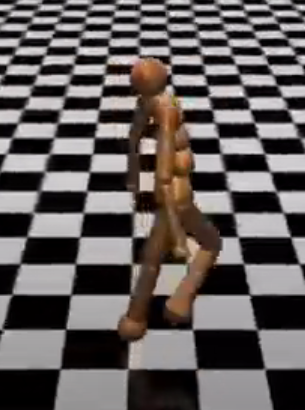
\includegraphics[width=.3\textwidth, height=0.4\textheight]{figures/rllab/Humanoid-v1.PNG}\hfill
    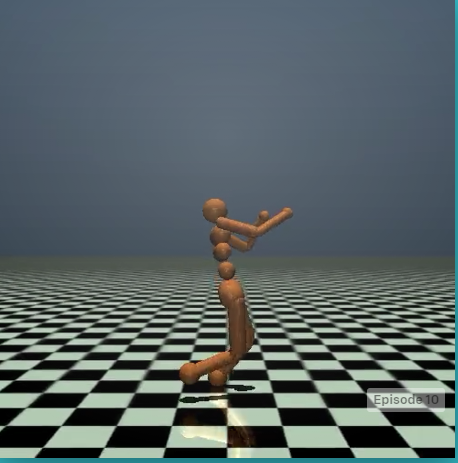
\includegraphics[width=.3\textwidth, height=0.4\textheight]{figures/rllab/Humanoid-v2.PNG}\hfill
    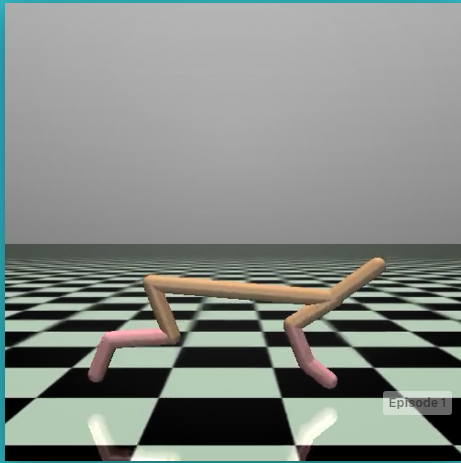
\includegraphics[width=.3\textwidth, height=0.4\textheight]{figures/rllab/halcheeathPNG.PNG}

    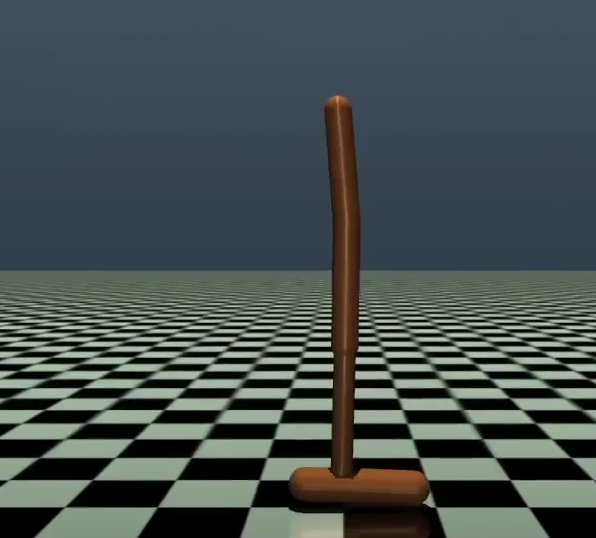
\includegraphics[width=.3\textwidth, height=0.4\textheight]{figures/rllab/Hopper.PNG}\hfill
    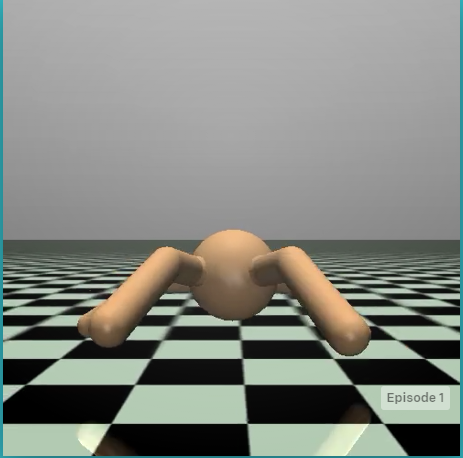
\includegraphics[width=.3\textwidth, height=0.4\textheight]{figures/rllab/antv2.PNG}\hfill
    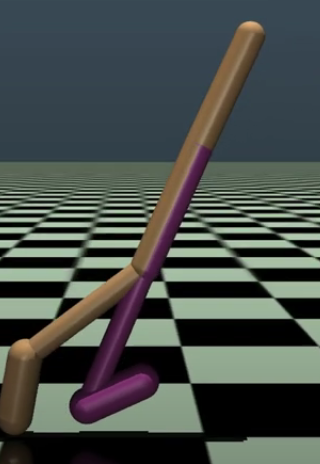
\includegraphics[width=.3\textwidth, height=0.4\textheight]{figures/rllab/walker.PNG}\hfill \\
    \cite{picturesrllab}
\end{frame}


\subsection{Vergleich mit anderen Algortihmen}
\note{
    DDPG = Deep Deterministic Policy Gradiend 
    TD3 =  Twin deep Deterministic gradiend
    PPO = Proximal Policy Optimization
}
\begin{frame}
    \frametitle{Ergebnisse}
    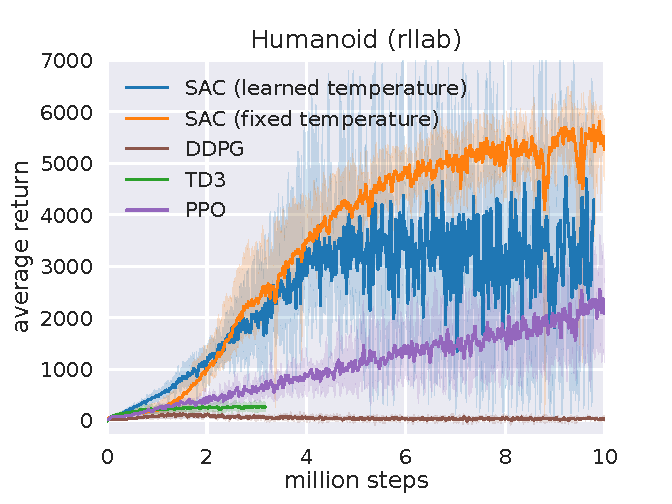
\includegraphics[width=.3\textwidth]{figures/humanoid-rllab.pdf}\hfill
    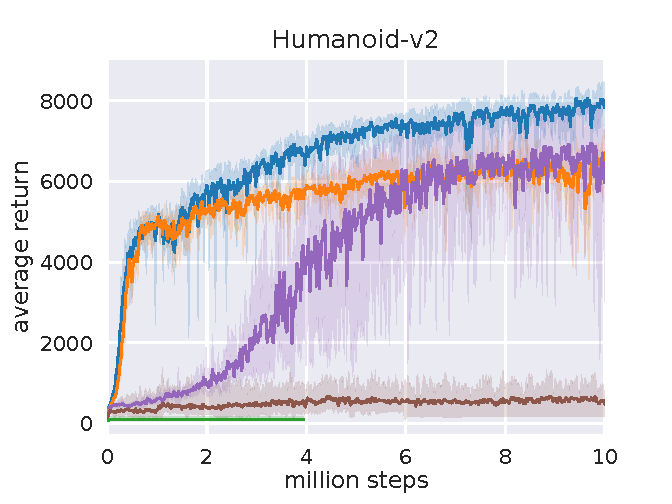
\includegraphics[width=.3\textwidth]{figures/humanoid-gym.pdf}\hfill
    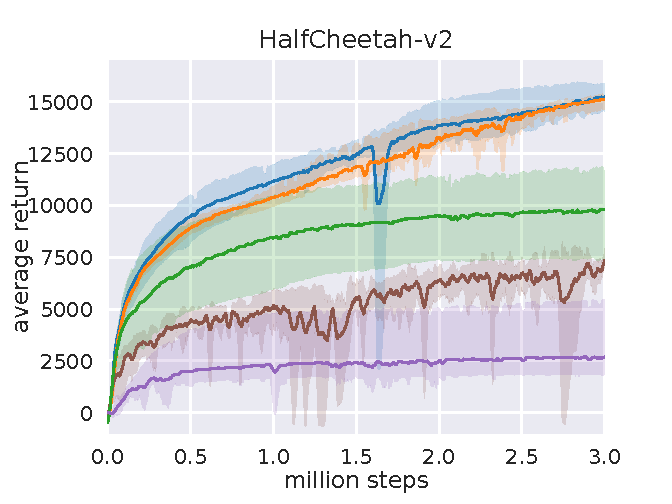
\includegraphics[width=.3\textwidth]{figures/half-cheetah.pdf}

    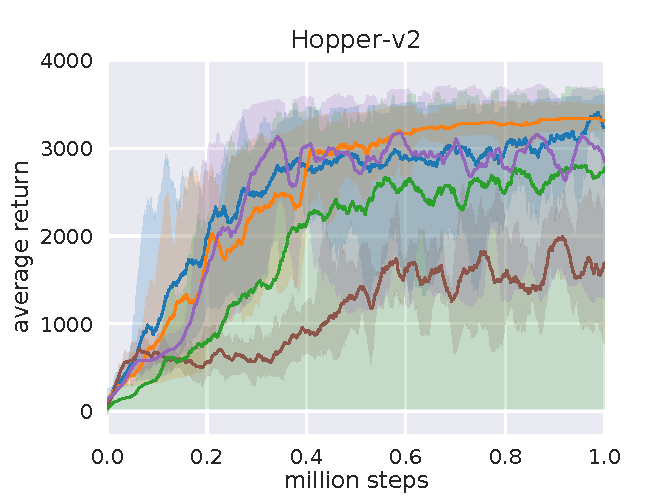
\includegraphics[width=.3\textwidth]{figures/hopper.pdf}\hfill
    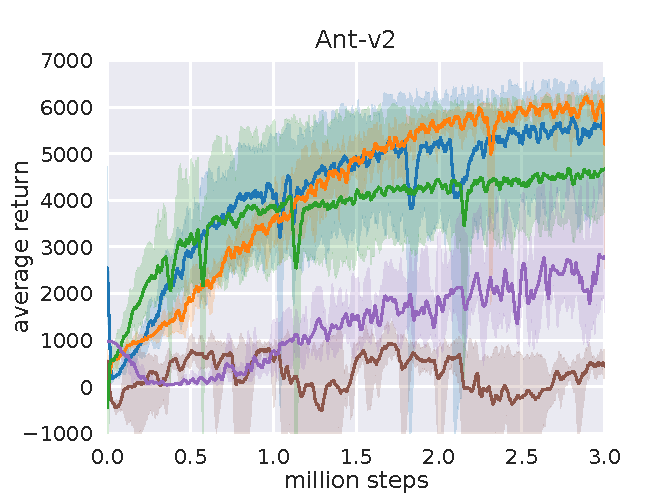
\includegraphics[width=.3\textwidth]{figures/ant.pdf}\hfill
    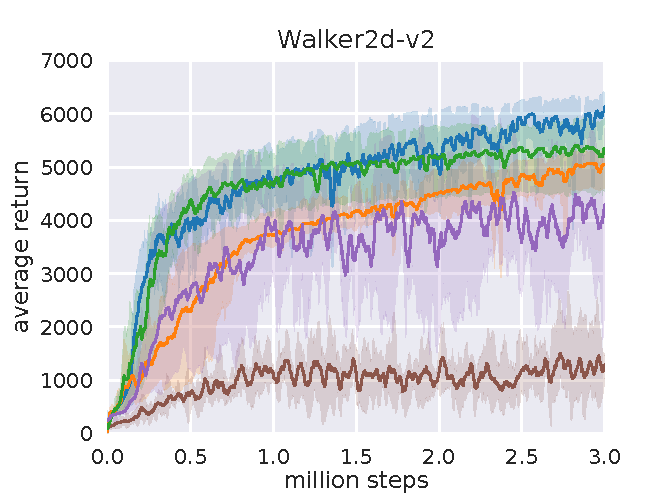
\includegraphics[width=.3\textwidth]{figures/walker.pdf}\hfill
    \cite{SAC19}
\end{frame}

%\begin{frame}
%    \frametitle{Ergebnisse}
%    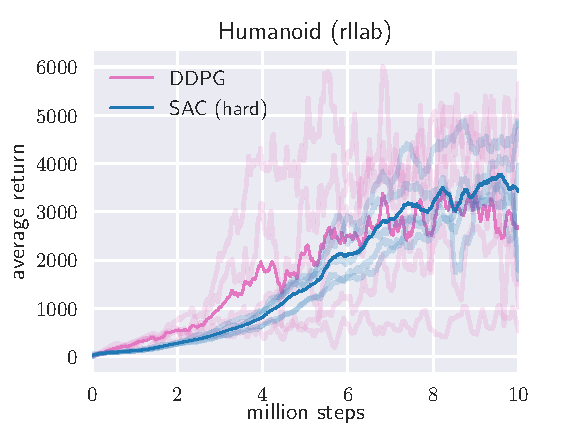
\includegraphics[width=0.8\textwidth]{figures/seeds-humanoid.pdf}
%\end{frame}


\subsection{Zusammenfassung}
\begin{frame}{Zusammenfassung}
        \begin{itemize}
            \item Soft actor critic vorgestellt
            \begin{itemize}
                \item Off policy Algorithmus
                \item Entropiemaximierung verbessert Stabilität
                \item Besser als state-of-the-art Algorithmen 
                \item Gradientenbasiertes Temperatur Tuning
            \end{itemize} 
        \end{itemize}
\end{frame}

	%Thilo	-5 bis Ende

\section{Conclusion}
\begin{frame}
    \frametitle{Conclusion}
    \begin{itemize}    
        \item Was haben wir bisher gesehen
        \item Performance im Vergleich zu TD3 und A2C
        \item Vor- und Nachteile von SAC
    \end{itemize}

\end{frame}

\end{document}